\section{Effektive Masse - Rückblick auf Mikro 1+2}
Die Beschreibung der Eigenleitung wird unter der Annahme getroffen, dass ein Elektron sich frei im Kristallgitter bewegen könne. Tatsächlich wirken aber innere Kräfte des Kristallgitters auf das Elektron. Diese Wirkung wird durch die Einführung einer effektiven Masse kompensiert.
	\begin{equation}
		m^* = \underbrace{\alpha}_{const.} \cdot \underbrace{m_0}_{Elektr. Masse} \qquad ,\; \alpha < 1,\; \text{materialabhängig}
	\end{equation}
	
	\section{Bandstruktur}
	Es existieren 2 Arten von Bandstruktur, zum einen die bekannte elektrische Bandstruktur, zum anderen die photonische Bandstruktur, über die z.B. ein Halbleiter unter Lichteinfluss beschrieben werden kann. Grundsätzlich muss aber beachtet werden, dass die Bandstruktur ein menschengemachtes Werkzeug ist um die Vorgänge im Material zu visualisieren und begreifen zu können. Folgend einige Graphiken unterschiedlicher Darstellungsmöglichkeiten der Vorgänge im Halbleiter:
\begin{figure}[H]
	\begin{minipage}{.5\linewidth}
		\centering
		\subfloat[]{\label{main:a}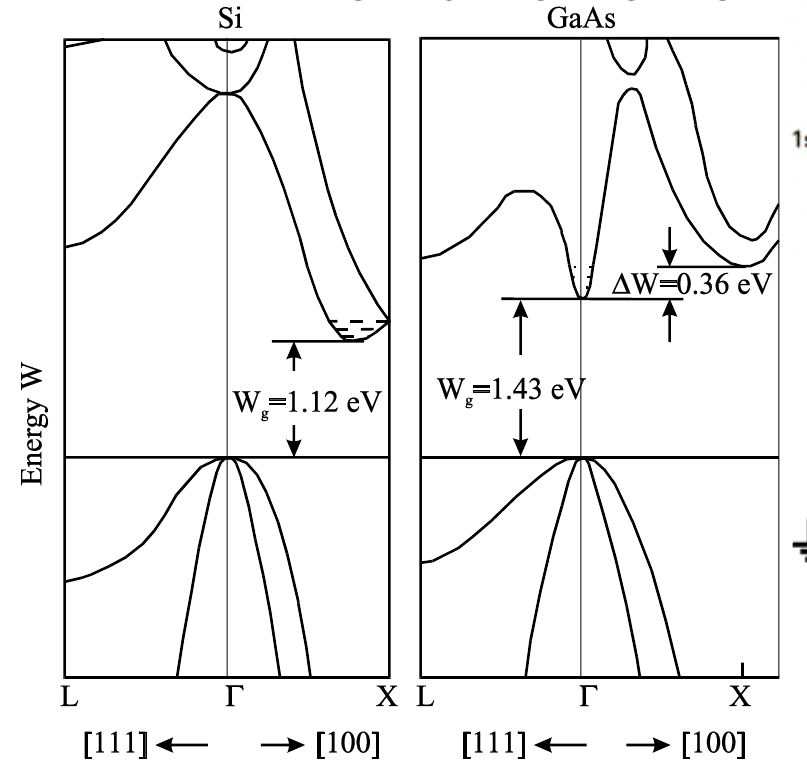
\includegraphics[scale=.2]{./img/bandstr_ul.png}}
	\end{minipage}%
	\begin{minipage}{.5\linewidth}
		\centering
		\subfloat[]{\label{main:c}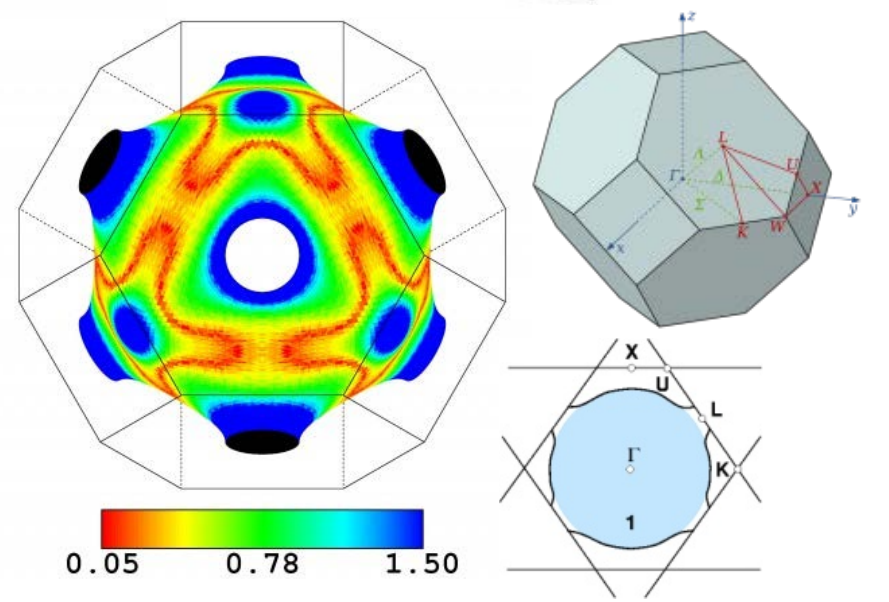
\includegraphics[scale=.2]{./img/bandstr_or.png}}
	\end{minipage}\par\medskip
	\centering
	\subfloat[]{\label{main:b}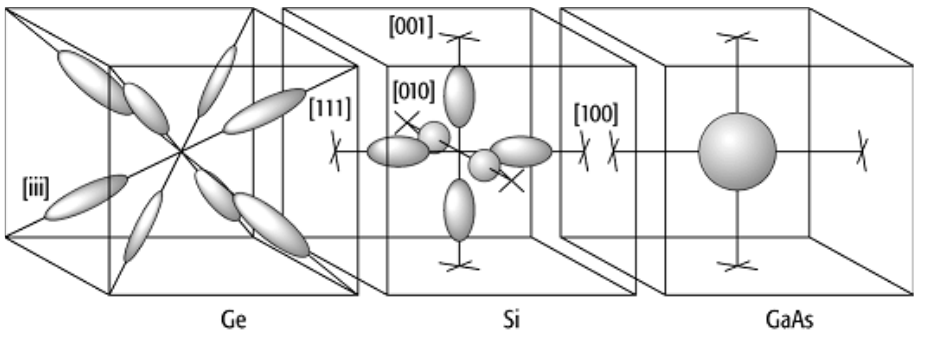
\includegraphics[scale=.23]{./img/bandstr_ur.png}}
	\caption{Einzelimpuls \protect\cite{HL1}}
\label{fig:main}
\end{figure}

(a) ist eine geschickte 2-dimensionale Darstellung von (c). Die in eckigen Klammern angegebenen Zahlenkombinationen nennt man Miller Indizies. (b) zeigt die Fermi-Fläche von Kupfer.

\section{Halbleitertypen}
	\subsection{Halbleiter und Metalle}
	\begin{itemize}
		\item Metalle sind grundsätzlich Kaltleiter $\rightarrow$ $T=0K \; \Rightarrow \; \sigma_M \rightarrow \infty$
		\begin{itemize}
			\item T $\uparrow \Rightarrow \sigma_M \downarrow, \; \sigma_M >>0$
		\end{itemize}
		\item Halbleiter sind grundsätzlich Heissleiter
		\begin{itemize}
			\item $T\uparrow \Rightarrow \sigma_{HL} \uparrow, \text{ aber } \sigma_{HL} << \sigma_M$
		\end{itemize}
	\end{itemize}
	
	\subsection{Elementhalbleiter} \label{ss_hltyp_ehl}
	Elementhalbleiter sind Halbleiter die nur aus einem Element bestehen.
	\subsection{Verbindungshalbleiter} \label{ss_hltyp_vhl}
	Verbindungshalbleiter sind immer 50/50 aufgeteilt, d.h. am Beispiel eines GaN (Galliumnitrid) III-V Verbindungshalbleiter ist das Kristallgitter so aufgebaut dass au jedes Galliumatom ein Stickstoffatom und dann wieder ein Galliumatom folgt. 
	\subsection{Legierungshalbleiter} \label{ss_hltyp_lhl}
	Legierungshalbleiter sind im Gegensatz zu Verbindungshalbleiter beliebig mischbar. Grundsätzlich sind alle Verhältnisse denkbar die sich ineinander lösen lassen.So können auch Kristallgitter entstehen, in denen gleiche Atome direkt benachbart sind.
	
\section{Bindungsarten}
	\subsection{Elektronenpaarbindung}
	Die zentrale Bindung bei Halbleitern ist die kovalente Bindung (auch Elektronenpaarbindung genannt). Aus \ref{ss_hltyp_lhl} und \ref{ss_hltyp_ehl} erkennt man damit, dass bei Verbindungshalbleitern nur kovalente Bindungen zwischen unterschiedlichen Atomen vorkommen kann, also am Beispiel von vorher nur kovalente Bindungen zwischen Gallium udn Stickstoff. Bei Legierungshalbleitern können dagegen auch kovalente Bindungen zwischen selben Atomen vorkommen, zum Beispiel Si-Si (Silizium) oder Ca-Ca (Cadmium) kovalente Bindungen.
	Kovalente Bindungen basieren auf dem Spin der äusseren Elektronen. Da bei der kovalenten Bindung beide Elektronen von jeweils beiden Atomen als äussere Elektronen beansprucht werden müssen die Spins entgegengesetzt sein. Damit ist das magnetische Moment entgegengesetzt wodurch eine magnetische Bindung entsteht. 
	\subsection{Metallische Bindung}
	Bei einem Metall gehört jedes Valenzelektron zu sehr vielen Atomen, somit verteilt sich die Bindung über das gesamte Volumen. Man kann sich ein Metall strukturell als Raumgitter aus vielen positiven Ionen vorstellen, zwischen denen sich ein frei bewegliches Elektronengas befindet. Diese freien Elektronen bilden somit eine negative Ladungswolke. Die Wechselwirkung aus der negativen Ladungswolke und den positiven Gitterionen sind Grundlage für die metallische Bindung. Typischerweise gibt jedes Atom ein bis zwei Atome in das Elektronengas, auch Fermi-Gas oder Fermi-See genannt, ab. Damit kann man direkt abschätzen, dass die Anzahl freier Elektronen zwar von Metall zu Metall variiert, aber in der Größenordnung immer ähnlich zur Anzahl der Atome sein muss.
	\subsection{Ionische Bindung}
	Grundsätzlich sind Atome bestrebt Edelgaskonfiguration anzunehmen, d.h. ihre äußerste Schale mit 8 Aussenelektronen zu besetzen. Eine ionische Bindung kommt dann besonders leicht zustande, wenn ein Atom zum Beispiel Natrium ein Aussenelektron in der äußersten Schale hat in räumliche Nähe zu einem weiteren Atom kommt dem gerade ein Aussenelektron zur Edelgaskonfiguration fehlt, z.B. Chlor. Gibt das Natrium sein Aussenelektron ab so ist die "neue" äußerste Schale gerade voll besetzt. Nimmt Chlor das abgegebene Elektron auf, so ist seine äußerste Schale auch gerade voll besetzt. Das Natriumatom wird damit zu einem positiv geladenen Natriumion, das Cloratom zu einem negativ geladenen Chloridion, die beide in Edelgaskonfiguration sind. Diese Verbindung heißt Natriumchlorid. Eine ionische Bindung kann aber auch in der Form vorliegen dass ein Atom mehrere Elektronen in der äußersten Schale hat. Aluminium hat zum Beispiel 3 Elektronen in der äußersten Schale, die es abgeben müsste um Edelgaskonfiguration zu erreichen. Es wäre dann ein 3-fach positiv geladenes Aluminiumion. Um diese Konfiguration zu erreichen muss es sich mit 3 Chloratomen verbinden, da jedes Chloratom bestrebt ist nur ein Elektron aufzunehmen. Die so entstandene Verbindung heißt Aluminiumchlorid.